\chapter{Simple substitution method}
\addcontentsline{toc}{chapter}{Simple substitution method}

In this chapter\footnote{This chapter is based on the article \citep{barancikova:2014},
joint work with Rudolf Rosa and Ale\v{s} Tamchyna.\todo{ Rudolf did all experiments with 
Depfix and Ale\v{s} was in charge of alignments}}, we present a basic algorithm 
for lexical (one-word) and phrase substitution based on phrasal alignment and tables 
of~synonymous expressions. \todo{Further, we apply Depfix -- the system originally designed 
for automatic correction of~grammatical errors that appear often in English-to-Czech 
MT outputs, on newly created paraphrases.} 

This method is independent on the evaluation metric. We use BLEU score in our 
experiments because of its common usage. Using our new reference sentences, 
BLEU achieves  significant improvement of its correlation with human judgment.

The algorithm is inspired by \cite{kauchak}, however, it differs in several aspects. 
As Czech belongs among~inflective languages with rich morphology, a Czech 
word has typically many forms and the correct form depends heavily on its 
context, e.g., cases of nouns depend on verb valency frames. Therefore, we do 
not attempt to~change a~single word in~a~reference sentence but we focus 
on~creating one single correct reference sentence.

Instead of the contextual evaluation, we focus on keeping grammatical correctness 
and the original meaning by using Depfix \citep{depfix} -- an automatic post-editing 
system which is able to fix Czech sentences containing grammatical errors.
\todo{Depfix was originally designed for post-editing outputs of English-to-Czech 
phrase-based machine translation. We adapted it to fit our setting.}

Furthermore, \cite{kauchak} use English WordNet as their source of paraphrases.
As~the Czech WordNet \citep{czech-wordnet,} is substantially smaller, we exploit --  
in~addition to~this language source --  Czech Meteor tables \citep{meteor07}. Because
of the noise in Czech Meteor tables, we experiment with adding alignment between 
the hypothesis and the corresponding reference sentence.

\begin{table}[t]
\begin{center}
\begin{tabular}{l|cc}
& WMT12 & WMT13 \\
\hline
WordNet            &  780 & 650 \\
filtered Meteor    & 4588 & 3877 \\
their union        & 4766 & 4013 \\
\end{tabular}
\caption{Average number of~pairs of~words identified as~a~paraphrase between 
a~MT output and a~corresponding reference sentence according to~their source.}
\label{number_of_substitutions}
\end{center}
\end{table}

\section{Algorithm}
We experiment with several algorithms for paraphrasing reference sentences. 
They differ in the method for selecting potential paraphrase pairs and in the 
length of paraphrases.

\subsection{Candidate Selection}
We select potential paraphrases using two different methods. The first one is a 
simple greedy search similar to~\citet{kauchak}, the other one uses automatic word
alignment for selecting corresponding segments of~the reference sentence and the 
hypothesis.

\subsubsection{Simple Greedy Method}
We perform morphological analysis and tagging of the MT outputs and
the reference sentences using Morče \cite{morce:2007}. \todo{premistit, kam se hodi}

Let $ W_{L} $, $ R_{L} $ be sets of lemmas
from the hypothesis (MT output) and the reference sentence, respectively. Then, one-word
paraphrase candidates are chosen as:

\begin{equation*}
C_{L} = \{(r,w) \, | \, r \in R_{L} \setminus W_{L} \wedge w \in W_{L} \setminus R_{L} \} 
\end{equation*}

Multi-words candidates $ C_M $ are selected as the Cartesian product of all sequences
from the reference sentence and all sequences from the hypothesis. Formally:

Let $ r_1,..., r_n $, $ w_1,...,w_m $ be the hypothesis and the reference sentence,
respectively. Then the set of multi-word paraphrase candidates is selected the following
way:

\begin{align*}
  C_{M} = \{ (<r_i,..,r_{i+x}>,<w_j,...,w_{j+y}>) \, | \, 1 \leq i \leq n-x \, \wedge \\ 
    \: 1~\leq~j \leq m-y  \: \wedge \: 0 \leq x,y \leq 6 \: \wedge \: (x \neq 0 \vee y \neq 0) \}
  \end{align*}

Maximum phrase length is seven words, which corresponds to the length of~the 
longest paraphrases in the paraphrase tables used in this experiment.

\subsubsection{Word and Phrase Alignments}

One possible way to make the algorithm more reliable is to restrict the
application of paraphrases to words/phrases which are aligned to each other. 
We compute word alignment between the reference translation and MT system
outputs using GIZA++ \citep{gizapp}.

If we used only our test data to create the alignment (13 x 3003 + 12 x 3000 
= 75039 sentence pairs), the alignment quality would be insufficient. In order 
to make the training data for word alignment larger, we take advantage of the 
fact that all outputs are translations of the same data and also add all pairs 
of system outputs to our data, creating over 1,000,000 \equo{artificial} sentence
pairs. For example, the parallel data for WMT12 then looks as follows:

\begin{center}
\begin{tabular}{ll}
Source & Target \\
\hline
system 1 & system 2 \\
system 1 & system 3 \\
... & ...\\
system 1 & system 13 \\
system 1 & reference \\
system 2 & system 1 \\
system 2 & system 3 \\
... & ... \\
system 13 & reference \\
\end{tabular}
\end{center}

We also experiment with adding much larger synthetic parallel data created by
machine translation (note that we need Czech-Czech data) but there was no impact
on the quality of paraphrasing so we follow the outlined approach which requires
no additional data or processing.

The set of~one-word candidates $C_L$ is then simply the set of all word pairs such
that there exists an alignment link between them. The set $C_M$ is extracted
using phrase extraction for phrase-based MT, the standard consistency criterion
is~applied \citep{Och99improvedalignment}.

\subsection{Paraphrasing}
We reduce the set $ C_{L} $ to pairs appearing in our paraphrase tables in the 
following way. If a word appears in several synonymous pairs we give preference 
to those found in~WordNet or even better in the intersection of paraphrases 
from WordNet and filtered Meteor. Similarly, we filter $ C_{M} $ to pairs also 
contained in the multi-word Meteor tables.

We evaluate three different paraphrasing methods which differ in the order of
substitution.

\begin{description}
\item[One-word only] We proceed word by word from the beginning of the 
reference sentence to~its end. If a~lemma of~a~word appears as~the first member 
of~a~pair in reduced $ C_{L} $, it is replaced by~the word from hypothesis that has 
its lemma as the second element of~that pair, i.e., paraphrase from the hypothesis. 
Otherwise, we keep the original word from the reference sentence.
\item[One-word first] We use \textit{One-word only} and then we apply longer 
paraphrases. In that case we move ahead from the longest paraphrases to the 
shortest. That is because Meteor contains often even components of~phrases 
and we could substitute, instead of~whole phrase, only part of~it. We do not 
attempt to replace any word that was already changed before.
\item[Multi-word first] We substitute the longest confirmed paraphrases from
$ C_{M} $ and move to the shorter ones. We replace again only sequences that 
have not been substituted yet. After this, we paraphrase the remaining 
unchanged words with the \textit{One-word only} method.
\end{description}

\subsection{Depfix}

Depfix is an automatic post-editing system, originally designed for improving quality
of phrase-based English-to-Czech machine translation outputs. It consists of a
set of~linguistically-motivated rules and a statistical component that correct
various kinds of errors, especially in grammar (e.g. morphological agreement),
using a range of natural language processing tools to provide analyses of the
input sentences.
% Tady bych src vlastně asi vůbec nepotřeboval, ty opravy co dělám ho přímo
% nevyužívaj, spíš jen pro kontrolu toho jestli analýza češtiny je rozumná;
% ale to by nebylo potřeba kontrolovat kdyby se analyzovala ta reference
% předtim než ji Petra zparafrázuje.
%It relies heavily on the availability of the source English
%sentences, which provide additional information both for the analyses and for
%the error correction.

We observe that the errors that appear in the outputs of our paraphrasing
algorithm are often similar to some errors appearing in outputs of phrase-based
machine translation systems, e.g errors in morphological agreement are very common.
This makes Depfix a good fit for fixing the errors, since typical
grammar correcting tools, such as a grammar-checker in a word processor,
focus on errors that are typical for humans, not for machines.

Also, the fact that Depfix exploits the source English sentences is an advantage 
in our case, as opposed to other grammar correcting tools, such as a 
grammar-checker in a word processor, which typically do not have access to an 
English translation and therefore do not use it to improve their performance.
For this reason, we apply Depfix post-editing to fix the errors in grammar that 
frequently appear in our outputs.

However, some error types that are common in phrase-based machine translation, 
such as errors in preserving the correct verb tense, do not frequently emerge in the 
paraphrasing process.
Therefore, we experiment with two Depfix configurations in this work:
\begin{description}
\item[full] the original Depfix system with all 33 fixing blocks,
as~described in \cite{rosa:mgr}
\item[limited] Depfix adapted for fixing paraphrasing errors by~disabling 10 of
the fixing blocks\footnote{%
The following fixing blocks are disabled in limited Depfix:
Fixing reflexive tantum,
Fixing morphological number of nouns,
Translation of \equo{by}, 
Translation of \equo{of}, 
Translation of present continuous,
Subject categories projection,
Missing reflexive verbs,
Subject personal pronouns dropping,
Tense translation,
Negation translation}
\end{description}

\begin{figure}[ht]
\begin{center}
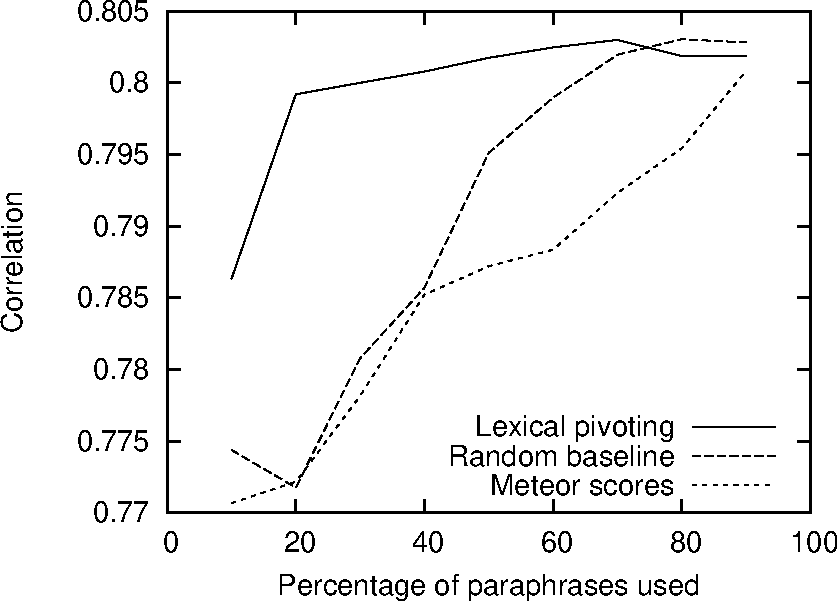
\includegraphics[scale=0.55]{../img/filtering-lexical-cropped.pdf}
\caption{Comparison of automatic filtering techniques for~\emph{one-word} paraphrases on WMT12 data.}
\label{fig:filtering-lexical}
\end{center}
\end{figure}

\begin{figure}[ht]
\begin{center}
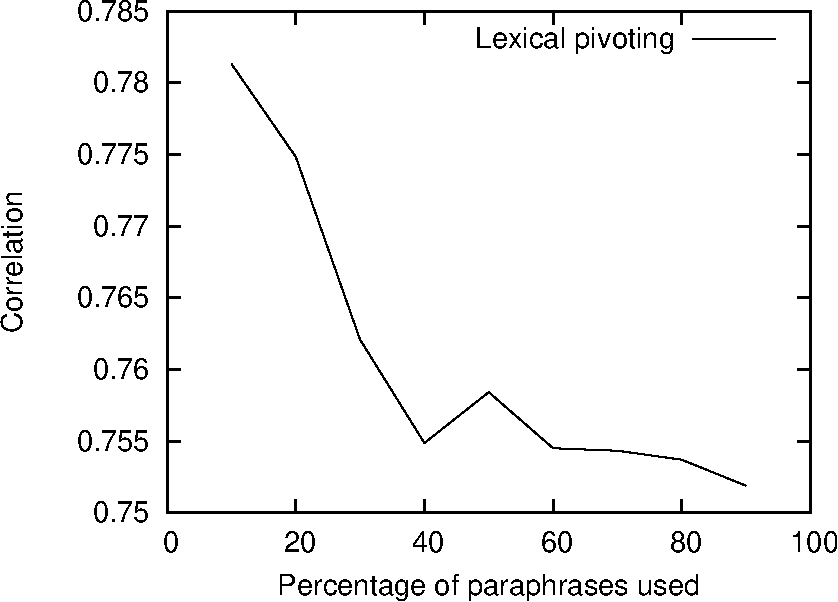
\includegraphics[scale=0.55]{../img/filtering-mwe-cropped.pdf}
\caption{Automatic filtering of multi-word paraphrase for~the \textit{multi-word-first} scenario on WMT12 data.}
\label{fig:filtering-mwe}
\end{center}
\end{figure}

\section{Filtering the Meteor Tables}
\label{filtering-section}

We try to remove the noise from the data with two different methods. The first
one is based on manual error analysis and it is applied to~one-word pairs only.
The second one is fully automatic and can be applied on all data, but its results are inconclusive.
Therefore, we employ only the first method in the rest of our experiments.

\subsection{Error-analysis Based Filtering}

We manually examine sentences after paraphrasing using only Meteor tables. Based on
our observation, we perform the following operations on pairs of one-word paraphrases 
from the Meteor tables:

\begin{itemize}
\item morphological analysis using Morče \citep{morce:2007} and replacing of word forms with their lemmas; 
\item removing pairs of identical lemmas;
\item removing pairs with different part of speech;
\item removing pairs of unknown words (typically foreign words).
\end{itemize}

The last two rules have a single exception -- paraphrases consisting of numeral and 
corresponding digits, e.g., \textit{osmnáct} (eighteen) and \textit{18}.\footnote{
\textit{0smnáct} has the part of speech \textit{C}, which is designated for numerals, 
\textit{18} is marked with \textit{X} meaning it is an unknown word for the morphological
analyzer.}
These paraphrases are very common in the data. 

This way we reduce more than 160 000 pairs of one word paraphrases to only 32 154
couples of lemmas. All examples of bad one-word paraphrases from Subsection \ref{meteori} 
are removed.

\subsection{Automatic Filtering}

Filtering strategies described in~this section are based on assigning a score to
each paraphrase pair. We then gradually remove paraphrases with low scores and
measure the effect on~the final correlation of~our metric.

The first, straightforward approach is to use the paraphrase scores already
provided in Meteor. They are based on~phrasal translation probabilities
and it corresponds to~paraphrase probability in~the pivoting model.

We propose an alternative scoring based on pivoting and lexical translation
scores:

$$\text{lex\_p}(\mathbf{s},\mathbf{t}) = \sum_{s \in \mathbf{s}}\sum_{t \in
\mathbf{t}}\sum_{pivot}\text{lex}(s|pivot)\text{lex}(pivot|t)$$

In this case, pivots are all words aligned to both $s$ and $t$ in the parallel
data. To get lexical translation probabilities, we use maximum likelihood
estimation from single best word alignment computed on CzEng 1.0
\citep{czeng10:lrec2012}. We refer to this score as \emph{lexical
pivoting}.

We use random selection as the baseline -- paraphrases are simply shuffled and we
then use the first 10, 20,$\ldots$ percent of them.

We only evaluate the filtering techniques on the WMT12 data. First, we attempt
to filter one-word paraphrases and use the cleaner paraphrase table in the
\emph{one-word-only} paraphrasing strategy. Note that our paraphrase table has
already been filtered using the error-analysis based filtering described above.

\Fref{fig:filtering-lexical} shows the performance of different filtering
techniques for one-word paraphrases. Relying on Meteor scores proves worse than
random selection. Using lexical pivoting, we can keep a high correlation even if we
throw away as much as 90\% of the paraphrases, however we do not improve 
(by~a~relevant margin) upon the baseline correlation of 0.802 achieved by
\emph{one-word-only} paraphrasing with the full paraphrase table.

We evaluate the best-performing technique also in the \textit{multi-word-first}
scenario where we use it for filtering multi-word paraphrases (see
\Fref{fig:filtering-mwe}). As we reduce the number of paraphrases, we observe a
considerable improvement of~correlation, however we never outperform
\textit{one-word-only} or \textit{one-word-first}. In this case, the filtering
simply mitigates the damage done by the multi-word paraphrases. We
cannot hope to achieve a higher score without a~more fine-grained grip on what
a~good multi-word paraphrase is.

\section{Results}


\begin{table}[t]
\begin{center}
\begin{tabular}{l|cc|cc}
\multirow{2}{*}{Method} & \multicolumn{2}{c|}{Greedy selection} & \multicolumn{2}{c}{Word alignment} \\
& Words & Phrases & Words & Phrases \\
\hline
One-word only     & 1.59 & --   & 0.86 &  --  \\
One-word first    & 1.59 & 0.23 & 0.86 & 0.22 \\
Multi-word first  & 1.38 & 0.31 & 0.81 & 0.27 \\
\end{tabular}
\caption{Average number of replaced words/phrases per~sentence for each method on data from WMT12.}
\label{replaced12}
\end{center}
\end{table}

\begin{table}[t]
\begin{center}
\begin{tabular}{l|cc|cc}
\multirow{2}{*}{Method} & \multicolumn{2}{c|}{Greedy selection} & \multicolumn{2}{c}{Word alignment} \\
& Words & Phrases & Words & Phrases \\
\hline
One-word only    & 1.33 &  --  & 0.76 & --   \\
One-word first   & 1.33 & 0.20 & 0.76 & 0.20 \\
Multi-word first & 1.04 & 0.68 & 0.74 & 0.24 \\
\end{tabular}
\caption{Average number of replaced words/phrases per~sentence for each method on data from WMT13.}
\label{replaced13}
\end{center}
\end{table}


\begin{table*}[tb]
\begin{center}
\begin{tabular}{l|ccc|ccc}
\multirow{2}{*}{Method} & \multicolumn{3}{c|}{Greedy selection} & \multicolumn{3}{c}{Word alignment} \\
& No Depfix & Full Depfix & Limited Depfix & No Depfix & Full Depfix & Limited Depfix\\
\hline
One-word only     & 0.802 & 0.827 & \textbf{0.832} & 0.792 & 0.813 & 0.810 \\
One-word first    & 0.785 & 0.822 & 0.816 & 0.767 & 0.792 & 0.798 \\
Multi-word first & 0.768 & 0.810 & 0.804 & 0.761 & 0.781 & 0.778 \\
\end{tabular}

\vspace{10pt}

Baseline~correlation: \textbf{0.749}
\caption{Correlation of the human judgment and BLEU computed with the data from WMT12}
\label{corrs12}
\end{center}
\end{table*}

\begin{table*}[tb]
\begin{center}
\begin{tabular}{l|ccc|ccc}
\multirow{2}{*}{Method} & \multicolumn{3}{c|}{Greedy selection} & \multicolumn{3}{c}{Word alignment} \\
& No Depfix & Full Depfix & Limited Depfix & No Depfix & Full Depfix & Limited Depfix\\
\hline
One-word only     & 0.861 & \textbf{0.887} & 0.883 & 0.856 & 0.877 & 0.872 \\
One-word first    & 0.851 & 0.880 & 0.875 & 0.833 & 0.871 & 0.863 \\
Multi-word first  & 0.838 & 0.870 & 0.864 & 0.833 & 0.868 & 0.861 \\
\end{tabular}

\vspace{10pt}

Baseline~correlation: \textbf{0.829}
\caption{Correlation of the human judgment and BLEU computed with the data from WMT13.}
\label{corrs13}
\end{center}
\end{table*}
 

Results of our method are presented in Tables \ref{corrs12} and \ref{corrs13}. The~baseline 
(i.e., using the original reference sentences) has a correlation of 0.749, 0.829 
respectively. All evaluated approaches outperform it, the simplest one \textit{One-word only}
performs best (\Fref{example} shows an example of this method).

We use a freely available
implementation\footurl{http://www.cnts.ua.ac.be/~vincent/scripts/rtest.py} of
\citep{meng1992comparing} to determine whether the difference in correlation
coefficients is statistically significant. The test shows that BLEU performs
better with our reference sentences with 99\% certainty. 

\begin{figure}[t]

\begin{center}
\begin{tabular}{ll}
 Source &  \begin{tabular}{l}
  	\textit{The location alone is classic.} \\
	\end{tabular} \\
 \hline
 
 Hypothesis & \begin{tabular}{llll}
 			\textit{Samotné} & \textit{místo} & \textit{je} & \textit{klasické.} \\
 			Actual & place & is & classic \\
			\end{tabular} \\
 &  \begin{tabular}{l}
  	The place alone is classic. \\
	\end{tabular} \\

 \hline
 Reference & \begin{tabular}{llll}
 			\textit{Už} & \textit{poloha} & \textit{je} & \textit{klasická.} \\
 			Already & position & is & classic. \\
			\end{tabular} \\
 &  \begin{tabular}{l}
  	The position itself is classic. \\
	\end{tabular}  \\ 

 \hline
  New reference & \begin{tabular}{llll}
 			\textit{Už} & \textit{místo} & \textit{je} & \textit{klasická.} \\
 			Already & place & is & classic \\
			\end{tabular} \\
 &  \begin{tabular}{l}
  	*The place itself is classic. \\
	\end{tabular} \\
 \hline 
  Depfixed ref. & \begin{tabular}{llll}
 			\textit{Už} & \textit{místo} & \textit{je} & \textit{klasické.} \\
 			Already & place & is & classic \\
			\end{tabular} \\
 &  \begin{tabular}{l}
  	The place itself is classic. \\
	\end{tabular} \\
 \hline  
 
\end{tabular}
\caption{Example of the \textit{One-word only} method. The~hypothesis is grammatically 
correct and has very similar meaning as the reference sentence. The new reference is closer 
in wording to the hypothesis, but there is no agreement between the noun and adjective. 
Depfix resolves the error and the final reference is correct and much similar to~the hypothesis.}
\label{example}
\end{center}
\end{figure}

Multi-word paraphrases are very noisy and while they do bring the system outputs closer to the 
reference (the average BLEU score of the systems increases), they often propose non-equivalent 
translations or violate the correctness of the sentence, thus blurring the differences between 
systems.

When paraphrasing is restricted by word alignment, all methods perform worse. As
Tables \ref{replaced12} 
and \ref{replaced13} show, the number of applied paraphrases is much lower: while the proportion of correct 
paraphrases is higher, their amount is reduced too much and overall, our technique is harmed by 
this restriction. 

On the other hand, applying Depfix is always beneficial, with the positive effects ranging 
from 0.017 up to 0.042. This supports our assumption of the importance of grammatical correctness 
of the created references. However, the \textit{limited} version is not optimally chosen and
performs worse than the \textit{full} version in most cases.

Results on the data from WMT13 and WMT12 are very similar. Again, paraphrasing helps to increase
the accuracy of the evaluation, even though the differences on the WMT13 data are not as~big due 
to much higher baseline. This is also reflected in~the smaller amount of substitutions (see \Tref{replaced13}).

\section{Conclusion and Future Work}
%Big difference in meteor (mozna zkusit jeste nejakou statistiku, jak casto dochazelo
%k substituci z meteoru a jak casto dochazi k substituci z meteoru x wordnetu? aby bylo
%opravdu mozne, ze ta filtrace vyznamne prispela??
Our results confirm the positive impact of paraphrasing a~reference sentence on the
performance of the BLEU score. We~evaluate a number of approaches to paraphrasing.
The best results are achieved by the \textit{one-word only} greedy substitution method.
We achieve a statistically significant improvement in the evaluation of 
English-to-Czech MT. 

We illustrate several methods for reducing noise in a paraphrase corpus and
we confirm importance of grammar correctness of reference sentences in MT 
evaluation by the improvement of correlation after applying Depfix.

In the future, we plan to further increase the correlation by creating our own 
Czech paraphrase tables that would be larger than Czech WordNet, but less noisy 
than Czech Meteor Tables.

Another way to improve the performance of our system which we want to follow
is a further adaptation of the Depfix system to our task. We intend to
tune existing Depfix corrections, as well as to add new corrections specific
to our task. We would also like to devise a way of~informing Depfix which parts
of the sentences come from the reference and which come from the paraphrasing
to eliminate \equo{false positives}, i.e. Depfix attempting to correct words
that are unlikely to be incorrect.